\chapter{Latent Semantic Indexing}
\label{cap:latent-semantic-indexing}
\intro{Il capitolo descrive gli obiettivi dell'analisi della semantica latente, introduce le basi teoriche e accenna a come sono utilizzabili nel recupero dell'informazione.}\\

Prendiamo come esempio la seguente matrice termini-documenti:
\begin{equation*}
    \mathbf{A}=
    \begin{blockarray}{*{6}{c} l}
      \begin{block}{*{6}{>{$\footnotesize}c<{$}} l}
        $D_1$ & $D_2$ & $D_3$ & $D_4$ & $D_5$ & $D_6$ & \\
      \end{block}
      \begin{block}{[*{6}{c}]>{$\footnotesize}l<{$}}
        1 & 1 & \textbf{\underline{0}} & 1 & 0 & 0 \bigstrut[t]& internet \\
        1 & \textbf{\underline{0}} & 1 & 1 & 0 & 0 & web \\
        1 & 1 & 1 & 2 & 1 & 1 & surfing \\
        0 & 0 & 0 & 1 & 1 & 1 & beach \\
      \end{block}
    \end{blockarray}
  \end{equation*}

È evidente che i concetti della collezione sono 2: uno riguarda il mondo dell'informatica(web) e l'altro dello sport(surf): in questo caso internet e web sono sinonimi, mentre surf può avere più significati. Assumiamo quindi che i primi 4 documenti si riferiscano al mondo dell'informatica, mentre i primi due invece a quello dello sport. Vorremmo quindi che il termine web e il termine internet fossero considerati come presenti anche nei documenti $D_2$ e $D_3$ e passare quindi da $A$ alla matrice modificata $A'$:

  \begin{equation*}
    \mathbf{A'}=
    \begin{blockarray}{*{6}{c} l}
      \begin{block}{*{6}{>{$\footnotesize}c<{$}} l}
        $D_1$ & $D_2$ & $D_3$ & $D_4$ & $D_5$ & $D_6$ & \\
      \end{block}
      \begin{block}{[*{6}{c}]>{$\footnotesize}l<{$}}
        1 & 1 & \textbf{\underline{1}} & 1 & 0 & 0 \bigstrut[t]& internet \\
        1 & \textbf{\underline{1}} & 1 & 1 & 0 & 0 & web \\
        1 & 1 & 1 & 2 & 1 & 1 & surfing \\
        0 & 0 & 0 & 1 & 1 & 1 & beach \\
      \end{block}
    \end{blockarray}
  \end{equation*}

  In questo modo è possibile recuperare, per esempio, il documento $D_2$ anche cercando "web".
  Notiamo anche che il rango della matrice modificata è 2, mentre il rango della matrice originale è 4.
  Una base di $A'$ è infatti:
  \begin{equation}
    \mathbf{B} = \begin{pmatrix}
        1 & 0 \\
        1 & 0 \\
        1 & 1 \\
        0 & 1 \\   
    \end{pmatrix}
\end{equation}

La base $B$ è la matrice che rappresenta i concetti della matrice originale, mentre $D$ è la rappresentazione dei documenti nello spazio dei concetti, dove $A = B \cdot D$
Nel caso particolare, D vale quindi:

 \begin{equation*}
    \mathbf{D}=
    \begin{blockarray}{*{6}{c} l}
      \begin{block}{*{6}{>{$\footnotesize}c<{$}} l}
        $B_1$ & $B_1$ & $B_1$ & $B_1 + B_2$ & $B_1$ & $B_1$ \\
      \end{block}
      \begin{block}{[*{6}{c}]>{$\footnotesize}l<{$}}
        1 & 1 & 1 & 1 & 0 & 0 \\
        0 & 0 & 0 & 1 & 1 & 1 \\
      \end{block}
    \end{blockarray}
  \end{equation*}

\section{Obiettivo della LSI}
Dati $A$, $k$ tali che: 
\begin{itemize}
    \item  $A$: matrice termini documenti di dimensione $mxn$
    \item  $k <  rango(A)$
\end{itemize}
trovare $A'$ di rango $k$ tale che la differenza tra $A'$ e $A$ sia la più piccola possibile.

\begin{equation*}
 \mathbf{A'} = argmin_{A'_{m x n} \text{con rango k}} \norm{A - A'}
\end{equation*}

\section{Calcolare A'}
\begin{figure}
  \centering
  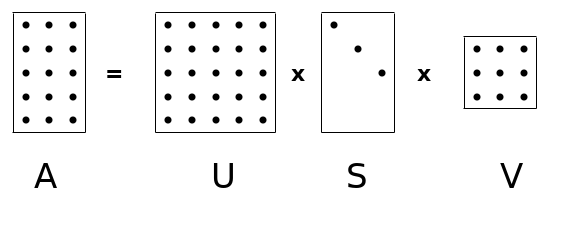
\includegraphics[scale=0.45]{immagini/SVD.png}
  \caption{Decomposizione ai valori singolari}
  \label{fig:calcoloSVD}
\end{figure}   

\begin{theorem}
Data una matrice A qualsiasi di dimensione $m x n$ e rango $k$, esistono $U$, $S$, $V$ tali che $A = U \cdot S \cdot V$ , dove:
\begin{itemize}
    \item $U$ è una matrice $m \cdot k$ con $U^T \cdot U = I_k$
    \item $S$ è una matrice diagonale $k \cdot k$
    \item $V$ è una matrice $k \cdot k$ con $V \cdot V^T = I_k$
\end{itemize}
\end{theorem}
Tale decomposizione è detta decomposizione ai valori singolari o SVD. Utilizzando la decomposizione ai valori singolari è quindi possibile calcolare il valore di $A$.

\noindent Posto $A = U \cdot S \cdot V$ la SVD di A:
\begin{itemize}
    \item $U_k$ = le prime $k$ colonne di $U$
    \item $S_k$ = la parte superiore $k \cdot k$ di $S$
    \item $V_k$ = le prime $k$ righe di $V$
\end{itemize}

e $A_k = U_k *  V_k * U_k$, allora $A' = A_k$, ovvero la matrice che minimizza $\norm{A - A'}$.

\section{Calcolare la SVD}
Il calcolo della decomposizione ai valori singolari si basa su una generalizzazione della \gls{edv}. La matrice $A$ termini-documenti è, infatti, una matrice rettangolare, mentre una precondizione per poter applicare la decomposizione agli autovettori è quella di avere una matrice quadrata.
Per quanto riguarda la libreria scelta per il calcolo della decomposizione, l'algoritmo attualmente implementato è quello di Golub-Kahan.\footnote{Questo emerge esaminando la libreria \url{https://github.com/lauerfab/MLweb/blob/92142d92abd64b12b251a43966d354328e3c9bbb/lalolab/src/linalg.js\#L6844}}

L'algoritmo di Golub-Kahan calcola la \gls{svd} in due passi:
\begin{enumerate}
    \item riduce la matrice a una matrice bidiagonale utilizzando una sequenza di trasformazioni di Householder;
    \item riduce la superdiagonale della matrice, utilizzando una sequenza di trasformazioni di Givens.
\end{enumerate} 

\section{Migliorare la ricerca utilizzando la LSI}
Per migliorare la ricerca utilizzando la \gls{lsi}, ci sono almeno 3 possibilità:
\begin{enumerate}
    \item utilizzare la matrice $A_k$ al posto della matrice $A$
    \item utilizzare la matrice $V_k$ al posto della matrice $A$
    \item espandere la matrice originale $A$.
\end{enumerate}